\documentclass[12pt]{article}
\usepackage{mathtools}
\usepackage[papersize={210mm, 270mm},tmargin=17mm,bmargin=15mm,lmargin=15mm,rmargin=15mm]{geometry}
\usepackage[utf8]{inputenc}
\usepackage{graphicx}
\usepackage{fancyhdr}
\pagestyle{fancy}
\lhead[\thepage]{David Cuesta Martín}
\rhead[David Cuesta Martín]{\thepage}
\cfoot{}
\author{David }


\begin{document}
\textbf{Ejercicio 1: }Como tenemos $R=\{(1,1),(1,2),(2,3),(3,4)\}$, tenemos la siguiente "matriz de adyacencia":\\
\begin{equation*}
    \begin{pmatrix}
    1 & 1 & 0 & 0 \\ 0 & 0 & 1 & 0 \\ 0 & 0 & 0 & 1 \\ 0 & 0 & 0 & 0 
    \end{pmatrix}
\end{equation*}
Por tanto, hacemos $R^2$ haciendo la multiplicación booleana de esta matriz de adyacencia:\\ 


\begin{equation*}
    \begin{matrix}
        1 \\ 2 \\ 3 \\ 4
    \end{matrix} 
    \begin{pmatrix}
    1 & 1 & 0 & 0 \\ 0 & 0 & 1 & 0 \\ 0 & 0 & 0 & 1 \\ 0 & 0 & 0 & 0 
    \end{pmatrix} \odot
    \begin{pmatrix}
    1 & 1 & 0 & 0 \\ 0 & 0 & 1 & 0 \\ 0 & 0 & 0 & 1 \\ 0 & 0 & 0 & 0 
    \end{pmatrix}=
    \begin{pmatrix}
    1 & 1 & 1 & 0 \\ 0 & 0 & 0 & 1 \\ 0 & 0 & 0 & 0 \\ 0 & 0 & 0 & 0 
    \end{pmatrix}
\end{equation*}
. \hspace{137px}1\ \ 2\ \ 3\ \ 4 \\ 
Esta matriz de adyacencia se corresponde a $R^2$. Para conseguir $R^3$ multiplicamos $R^2$ por $R$:
\begin{equation*}
    \begin{pmatrix}
    1 & 1 & 1 & 0 \\ 0 & 0 & 0 & 1 \\ 0 & 0 & 0 & 0 \\ 0 & 0 & 0 & 0 
    \end{pmatrix} \odot
    \begin{pmatrix}
    1 & 1 & 0 & 0 \\ 0 & 0 & 1 & 0 \\ 0 & 0 & 0 & 1 \\ 0 & 0 & 0 & 0 
    \end{pmatrix}=
    \begin{pmatrix}
    1 & 1 & 1 & 1 \\ 0 & 0 & 0 & 0 \\ 0 & 0 & 0 & 0 \\ 0 & 0 & 0 & 0 
    \end{pmatrix}
\end{equation*}
Por tanto, con la nueva matriz de adyacencia que obtenemos ya tenemos $R^3$.\\
\textbf{Solución: }\fbox{$R^3=\{(1,1),(1,2),(1,3),(1,4)\}$}\\ \\ 
Comprobamos con el script de Octave, y vemos que es correcto:\\ 

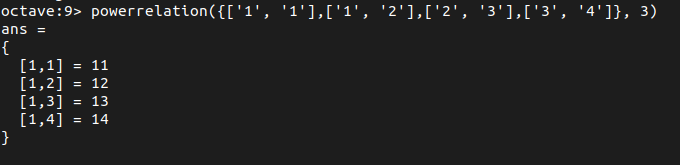
\includegraphics[width=15cm]{img1.png}
\end{document}
